% Source: Weinberg GR, physical PDF pp. 515--532
%         (printed pp. 491--506; boundary pages are partial).
%         Physical pp. 526/528 both reproduce printed p. 502, and
%         physical pp. 527/529 both reproduce printed p. 503; each repeated
%         printed leaf is transcribed once.
% Coverage: Section 15.4, Intergalactic Emission and Absorption Processes;
%           equations (15.4.1)--(15.4.50), including all unnumbered displays.
% Figures/tables/footnotes: Figure 15.2; reference notes 26--50c; no tables.
% Status: source-reviewed and compile-clean; visually proofed.
% Uncertainties: none.
% MODERNIZATION: R_{\mathrm{source}}(t) -> a(t), with a_0=a(t_0);
% H=\dot a/a and the existing modern q convention. Long coordinate
% derivatives are compacted where they occur. The source symbols N,
% \mathcal N, \Gamma, \Lambda, \Omega, and \Sigma are retained because they
% distinguish ray density, background spectral density, spontaneous emission,
% absorption, stimulated emission, and scattering.
% LITERAL-OPERATOR AUDIT: every leading sign and continuation operator in
% equations (15.4.1)--(15.4.50) was checked directly against physical PDF
% pp. 515--532, including the long transfer equations (15.4.9)--(15.4.14).

\subsection{Intergalactic Emission and Absorption Processes}\label{sec:15.4}

Up to now we have dealt only with light signals, which are emitted by distant
discrete sources, and propagate to us through essentially empty space. However,
we saw in Section~\ref{sec:15.2} that Einstein's equations require a cosmic
energy density (if \(H_0\simeq75\,\mathrm{km/sec/Mpc}\) and \(q_0\simeq1\))
about equal to \(2\times10^{-29}\,\mathrm{g/cm^3}\), which is some 70 times
larger than the observed density of galactic mass. If the missing mass takes the
form of an ionized or neutral gas filling intergalactic space, then we can hope
to measure the mass density, and distinguish between cosmological models, by
observing the absorption or time delay of light as it passes through the
intergalactic gas, or by observing the background radiation emitted by this
gas. The absorption of light signals, and the emission and absorption of
background radiation, become even more important when we turn our attention
back to the early universe, when the density and opacity of matter was
enormously greater than it is today.

To lay a foundation for our treatment of these problems, let us first consider
the effects of absorption and emission on a ray of light, which leaves a source
at time \(t_1\) with frequency \(\nu_1\), and arrives at the earth at time
\(t_0\). If no emission occurs in the intervening medium, then the loss of flux
of the light ray is given by an equation of form
\begin{equation}
  \dot N(t)
  =
  -\Lambda\left(\nu_1\frac{a(t_1)}{a(t)},t\right)N(t),
  \tag{15.4.1}\label{eq:15.4.1}
\end{equation}
where \(N\) is the photon number density in the light ray, and
\(\Lambda(\nu,t)\) is the absorption rate (per unit proper time) of light with
frequency \(\nu\). [It is implicitly understood here that at time \(t\) the
photons in the ray have red-shifted frequency
\(\nu_1a(t_1)/a(t)\).] The solution is usually written in the form
\begin{equation}
  N(t_0)=e^{-\tau}N(t_1),
  \tag{15.4.2}\label{eq:15.4.2}
\end{equation}
where \(\tau\) is the \emph{optical depth}:
\begin{equation}
  \tau
  =
  \int_{t_1}^{t_0}
  \Lambda\left(\nu_1\frac{a(t_1)}{a(t)},t\right)\dd t.
  \tag{15.4.3}\label{eq:15.4.3}
\end{equation}

Now suppose that the medium itself, apart from effects of the light ray,
isotropically emits \(\Gamma(\nu,t)\) photons per unit proper volume, per unit
proper time, and per unit frequency interval at frequency \(\nu\). These
photons do not become part of the light ray, but join the isotropic background
radiation, to be discussed below. However, Bose statistics require that photons
will be added to the light ray through the process of \emph{stimulated
emission},\hyperref[ch15-ref-26]{\textsuperscript{26}} at a rate, per photon
in the light ray, given rigorously by
\begin{equation}
  \Omega(\nu,t)=\frac{\Gamma(\nu,t)}{8\pi\nu^2}.
  \tag{15.4.4}\label{eq:15.4.4}
\end{equation}
In place of Eq.~\eqref{eq:15.4.2}, the rate of change of photon number density
in the light ray is now given by the formula
\begin{equation}
  \dot N(t)
  =
  -\Lambda\left(\nu_1\frac{a(t_1)}{a(t)},t\right)N(t)
  +\Omega\left(\nu_1\frac{a(t_1)}{a(t)},t\right)N(t),
  \tag{15.4.5}\label{eq:15.4.5}
\end{equation}
and so the optical depth in Eq.~\eqref{eq:15.4.2} must now be written as
\begin{equation}
  \tau
  =
  \int_{t_1}^{t_0}
  \left[
    \Lambda\left(\nu_1\frac{a(t_1)}{a(t)},t\right)
    -
    \Omega\left(\nu_1\frac{a(t_1)}{a(t)},t\right)
  \right]\dd t.
  \tag{15.4.6}\label{eq:15.4.6}
\end{equation}
If the medium is in thermal equilibrium, not necessarily in equilibrium with
radiation, then \(\Omega\) and \(\Lambda\) are related by the Einstein
formula\hyperref[ch15-ref-27]{\textsuperscript{27}}:
\begin{equation}
  \Omega(\nu,t)
  =
  \exp\left[-\frac{h\nu}{kT(t)}\right]\Lambda(\nu,t),
  \tag{15.4.7}\label{eq:15.4.7}
\end{equation}
where \(h\) is Planck's constant, \(k\) is Boltzmann's constant, and \(T(t)\)
is the temperature of the medium at time \(t\). [This result simply follows
from the principle of detailed balance. The rate of spontaneous emission of
photons per unit volume of phase space in any given transition within the
medium is equal to the rate of absorption of photons in the inverse transition,
times the ratio of the populations of the upper and lower states, which is
simply given by the Boltzmann factor \(\exp(-h\nu/kT)\). This factor depends
only on \(\nu\) and \(T\), so the total rate of spontaneous emission per unit
volume of phase space, which according to \eqref{eq:15.4.4} is just
\(\Omega\), is equal to the total absorption rate \(\Lambda\), times
\(\exp(-h\nu/kT)\).] The optical depth is then
\begin{equation}
  \tau
  =
  \int_{t_1}^{t_0}
  \left\{
    1-\exp\left[
      -\frac{h\nu_1a(t_1)}{kT(t)a(t)}
    \right]
  \right\}
  \Lambda\left(\nu_1\frac{a(t_1)}{a(t)},t\right)\dd t.
  \tag{15.4.8}\label{eq:15.4.8}
\end{equation}

Even if the medium is not strictly in thermal equilibrium, it is often a good
approximation to use \eqref{eq:15.4.7} and \eqref{eq:15.4.8}, with \(T(t)\)
taken as an \emph{effective temperature}. Normally, \(T\) is positive, so
\(e^{-\tau}<1\), and a light ray is weakened as it passes through the medium.
However, it is sometimes possible to have a population inversion in the
medium, with a negative effective temperature. In this case \(\tau\) is
negative, so \(e^{-\tau}>1\), and a light ray is amplified by the medium. Such
maser phenomena have been detected within our galaxy, but not yet in
intergalactic space.

Apart from the images of discrete sources, there is also an \emph{isotropic
background} of radiation produced by the universe as a whole. Let
\(\mathcal N(\nu_0,t)\dd\nu_0\) be the number density of photons at time \(t\),
which at time \(t_0\) would have frequency between \(\nu_0\) and
\(\nu_0+\dd\nu_0\). If no absorption or emission occurs, then by the same
reasoning that led to Eq.~\eqref{eq:14.2.17}, the time dependence of
\(\mathcal N(\nu_0,t)\) would simply be given by a factor \(a^{-3}(t)\),
arising from the general expansion of the universe. In order to calculate the
rate of change of \(\mathcal N(\nu_0,t)a^3(t)\) owing to spontaneous emission
processes, we note that photons, which at time \(t_0\) are in the frequency
range from \(\nu_0\) to \(\nu_0+\dd\nu_0\), are in the frequency range from
\(\nu_0a(t_0)/a(t)\) to
\((\nu_0+\dd\nu_0)a(t_0)/a(t)\) at time \(t\); hence the rate of change of
the number of photons \(\mathcal N(\nu_0,t)a^3(t)\dd\nu_0\) in a proper
volume \(a^3(t)\) and a frequency interval \(\dd\nu_0\) at \(t_0\) is
\[
  \Gamma\left(\nu_0\frac{a(t_0)}{a(t)},t\right)
  a^3(t)\left(\frac{a(t_0)\dd\nu_0}{a(t)}\right),
\]
where \(\Gamma\) is again the rate of spontaneous emission per unit proper
volume and per unit frequency interval, now including all discrete sources as
well as the medium itself. The rate of change of
\(\mathcal N(\nu_0,t)a^3(t)\dd\nu_0\) due to induced emission and absorption
is
\[
  \left[
    \Omega\left(\nu_0\frac{a(t_0)}{a(t)},t\right)
    -
    \Lambda\left(\nu_0\frac{a(t_0)}{a(t)},t\right)
  \right]
  \mathcal N(\nu_0,t)a^3(t)\dd\nu_0,
\]
just as in Eq.~\eqref{eq:15.4.5}. Hence the effect of spontaneous and induced
emission and absorption is to give \(\mathcal N(\nu_0,t)a^3(t)\) the rate of
change
\begin{align*}
  \frac{\dd}{\dd t}\left\{\mathcal N(\nu_0,t)a^3(t)\right\}
  &=
  \Gamma\left(\nu_0\frac{a(t_0)}{a(t)},t\right)a^2(t)a(t_0)
  \\
  &\quad+
  \left[
    \Omega\left(\nu_0\frac{a(t_0)}{a(t)},t\right)
    -
    \Lambda\left(\nu_0\frac{a(t_0)}{a(t)},t\right)
  \right]\mathcal N(\nu_0,t)a^3(t).
\end{align*}
Using \eqref{eq:15.4.4} for \(\Gamma\), the solution is
\begin{align*}
  \mathcal N(\nu_0,t)a^3(t)
  &=
  \exp\left\{
    -\int_{t_1}^{t}
    \left[
      \Lambda\left(\nu_0\frac{a(t_0)}{a(t')},t'\right)
      -
      \Omega\left(\nu_0\frac{a(t_0)}{a(t')},t'\right)
    \right]\dd t'
  \right\}
  \mathcal N(\nu_0,t_1)a^3(t_1)
  \\
  &\quad+
  8\pi\nu_0^2a^3(t_0)
  \int_{t_1}^{t}
  \exp\left\{
    -\int_{t'}^{t}
    \left[
      \Lambda\left(\nu_0\frac{a(t_0)}{a(t'')},t''\right)
      -
      \Omega\left(\nu_0\frac{a(t_0)}{a(t'')},t''\right)
    \right]\dd t''
  \right\}
  \\
  &\hspace{8em}\times
  \Omega\left(\nu_0\frac{a(t_0)}{a(t')},t'\right)\dd t',
\end{align*}
with \(t_1\) arbitrary. The first term just gives the number of photons left
over from before \(t_1\), and the second gives the number of photons emitted
since \(t_1\); in both cases the exponential factors represent the subsequent
effects of absorption and induced emission. This result simplifies if we take
\(t\) as the present instant \(t_0\), and take \(t_1\) sufficiently far in the
past so that essentially all the background radiation was emitted since then.
The present number density of photons per unit frequency interval is then
\begin{align}
  n_{\gamma0}(\nu_0)
  &\equiv\mathcal N(\nu_0,t_0)
  \notag\\
  &=
  8\pi\nu_0^2
  \int_{t_1}^{t_0}
  \exp\left\{
    -\int_t^{t_0}
    \left[
      \Lambda\left(\nu_0\frac{a(t_0)}{a(t')},t'\right)
      -
      \Omega\left(\nu_0\frac{a(t_0)}{a(t')},t'\right)
    \right]\dd t'
  \right\}
  \notag\\
  &\qquad\times
  \Omega\left(\nu_0\frac{a(t_0)}{a(t)},t\right)\dd t.
  \tag{15.4.9}\label{eq:15.4.9}
\end{align}
If the medium is in thermal equilibrium, then \eqref{eq:15.4.7} can be used to
express \(\Omega\) in terms of \(\Lambda\), and the present photon number
density becomes
\begin{align}
  n_{\gamma0}(\nu_0)
  &=
  8\pi\nu_0^2
  \int_{t_1}^{t_0}
  \exp\left[
    -\frac{h\nu_0a(t_0)}{kT(t)a(t)}
  \right]
  \Lambda\left(\nu_0\frac{a(t_0)}{a(t)},t\right)
  \notag\\
  &\quad\times
  \exp\left\{
    -\int_t^{t_0}
    \left[
      1-\exp\left(
        -\frac{h\nu_0a(t_0)}{kT(t')a(t')}
      \right)
    \right]
    \Lambda\left(\nu_0\frac{a(t_0)}{a(t')},t'\right)\dd t'
  \right\}\dd t.
  \tag{15.4.10}\label{eq:15.4.10}
\end{align}

We have not yet considered the effects of photon \emph{scattering}. In
calculating the optical depth of a discrete source, any sort of scattering will
remove photons from the light rays, with no stimulated emission to return
photons to the ray. Instead of \eqref{eq:15.4.8}, the optical depth will then
be
\begin{align}
  \tau
  &=
  \int_{t_1}^{t_0}
  \left\{
    1-\exp\left[
      -\frac{h\nu_1a(t_1)}{kT(t)a(t)}
    \right]
  \right\}
  \Lambda\left(\nu_1\frac{a(t_1)}{a(t)},t\right)\dd t
  \notag\\
  &\quad+
  \int_{t_1}^{t_0}
  \Sigma\left(\nu_1\frac{a(t_1)}{a(t)},t\right)\dd t,
  \tag{15.4.11}\label{eq:15.4.11}
\end{align}
where \(\Sigma(\nu,t)\) is the scattering rate for a photon of frequency
\(\nu\) at time \(t\). It is much more difficult to take into account the
effects of photon scattering on the isotropic background, because each
scattering contributes a photon to the background for every one it takes away.
The one case that is easily dealt with is Thomson scattering, in which both
\(h\nu\) and \(kT\) are much less than the charged particle mass. In such
scatterings, there is no change in the photon frequency, so the scattering
simply has no effect on the isotropic background. In our calculations of the
isotropic background, we shall have to assume that scattering, except for
Thomson scattering, is much rarer than absorption. (However, note that
resonant scattering must be counted as absorption, if the mean lifetime of the
resonant state is long compared with the mean free time of the particles in the
medium.)

Let us now apply this formalism to the problem of detecting the ``missing
mass'' in intergalactic space. If the intergalactic medium consists of a
rarefied gas of neutral atoms, such as hydrogen, then it will absorb radiation
strongly at various discrete frequencies, corresponding to various transitions
between atomic states. For simplicity, let us suppose that all absorption takes
place within a small frequency interval centered on a single absorption
frequency \(\nu_a\). The absorption rate is then of the form
\[
  \Lambda(\nu,t)=n(t)\sigma_a(\nu),
\]
where \(n(t)\) is the number density of atoms at cosmic time \(t\), and
\(\sigma_a(\nu)\) is the absorption cross-section, assumed to be negligible
except within a sharp peak at \(\nu_a\). According to \eqref{eq:15.4.8},
essentially all absorption of a ray of light, which leaves a source at time
\(t_1\) with frequency \(\nu_1>\nu_a\) and arrives here at time \(t_0\) with
frequency \(\nu_0<\nu_a\), will take place at a time \(t_a\) such that
\begin{equation}
  a(t_a)
  =
  \frac{\nu_1a(t_1)}{\nu_a}
  =
  \frac{\nu_0a(t_0)}{\nu_a},
  \tag{15.4.12}\label{eq:15.4.12}
\end{equation}
so that the optical depth is
\[
  \tau
  \simeq
  n(t_a)
  \left[
    1-\exp\left(-\frac{h\nu_a}{kT(t_a)}\right)
  \right]
  \int
  \sigma_a\left(\nu_1\frac{a(t_1)}{a(t)}\right)\dd t.
\]
By changing variables from \(t\) to
\(\nu=\nu_1a(t_1)/a(t)\), we find
\begin{equation}
  \tau
  \simeq
  n(t_a)
  \left[
    1-\exp\left(-\frac{h\nu_a}{kT(t_a)}\right)
  \right]
  \left[\frac{a(t_a)}{\dot a(t_a)}\right]I_a,
  \tag{15.4.13}\label{eq:15.4.13}
\end{equation}
where
\begin{equation}
  I_a\equiv\frac1{\nu_a}\int\sigma(\nu)\dd\nu,
  \tag{15.4.14}\label{eq:15.4.14}
\end{equation}
the integral being taken over a range of frequencies just large enough to
include the whole absorption line. The choice of a particular cosmological
model is necessary here only in order to determine the Hubble ``constant''
\(\dot a/a\) at time \(t_a\); according to Eqs.~\eqref{eq:15.3.3},
\eqref{eq:15.4.12}, and \eqref{eq:15.3.22}, this is
\begin{align}
  \frac{\dot a(t_a)}{a(t_a)}
  &=
  \frac{a(t_0)}{a(t_a)}H_0
  \left[
    1-2q_0+2q_0\frac{a(t_0)}{a(t_a)}
  \right]^{1/2}
  \notag\\
  &=
  \left(\frac{\nu_a}{\nu_0}\right)H_0
  \left[
    1-2q_0+2q_0\frac{\nu_a}{\nu_0}
  \right]^{1/2}.
  \tag{15.4.15}\label{eq:15.4.15}
\end{align}
Using \eqref{eq:15.4.15} in \eqref{eq:15.4.13}, we see that the optical
depth at a \emph{received} frequency \(\nu_0\) is
\begin{equation}
  \tau(\nu_0)
  \simeq
  \frac{\nu_0n(t_a)I_a}{\nu_aH_0}
  \left[
    1-\exp\left(-\frac{h\nu_a}{kT(t_a)}\right)
  \right]
  \left[
    1-2q_0+2q_0\frac{\nu_a}{\nu_0}
  \right]^{-1/2}.
  \tag{15.4.16}\label{eq:15.4.16}
\end{equation}
Of course, this result applies only when \eqref{eq:15.4.12} can be satisfied
along the light path, that is, for received frequencies in the range
\begin{equation}
  \frac{\nu_a}{1+z}\leq\nu_0\leq\nu_a,
  \tag{15.4.17}\label{eq:15.4.17}
\end{equation}
where \(z\equiv\nu_1/\nu_0-1\) is the red shift of the source. Therefore we
expect an \emph{absorption trough} in the received signal for \(\nu_0\) within
this range. The optical depth, caused by a single absorption line at frequency
\(\nu_a\), vanishes for \(\nu_0<\nu_a/(1+z)\), jumps up steeply at
\(\nu_a/(1+z)\) to a value
\begin{equation}
  \tau\left(\frac{\nu_a}{1+z}+\right)
  =
  \frac{n(t_1)I_a}{H_0(1+z)}
  \left[
    1-\exp\left(-\frac{h\nu_a}{kT(t_1)}\right)
  \right]
  [1+2q_0z]^{-1/2},
  \tag{15.4.18}\label{eq:15.4.18}
\end{equation}
then varies more or less smoothly until just below \(\nu_a\), where it takes
the value
\begin{equation}
  \tau(\nu_a-)
  =
  H_0^{-1}n(t_0)I_a
  \left[
    1-\exp\left(-\frac{h\nu_a}{kT(t_0)}\right)
  \right],
  \tag{15.4.19}\label{eq:15.4.19}
\end{equation}
and finally drops down sharply to zero for \(\nu_0>\nu_a\).

At the same time that the intergalactic medium is absorbing light signals, it
will also be emitting isotropic background radiation. If the medium has an
absorption line at frequency \(\nu_a\), then it will have a single emission line
at the same frequency, and the emitted radiation will be observed at
red-shifted frequencies \(\nu_0<\nu_a\). Using \eqref{eq:15.4.10}, and
following the same reasoning that led to \eqref{eq:15.4.16}, we find that the
present number density of background photons per unit frequency interval at a
received frequency \(\nu_0\) is
\begin{equation}
  \mathcal N(\nu_0,t_0)
  =
  \frac{8\pi\nu_0^3n(t_a)I_a}{\nu_aH_0}
  \exp\left(-\frac{h\nu_a}{kT(t_a)}\right)
  \left[
    1-2q_0+2q_0\frac{\nu_a}{\nu_0}
  \right]^{-1/2},
  \tag{15.4.20}\label{eq:15.4.20}
\end{equation}
with \(I_a\) and \(t_a\) given by \eqref{eq:15.4.14} and
\eqref{eq:15.4.12}, respectively. The background density \(\mathcal N\)
varies with \(\nu_0\) more or less smoothly up to just below the frequency
\(\nu_a\), where
\begin{equation}
  \mathcal N(\nu_a-,t_0)
  =
  8\pi\nu_a^2H_0^{-1}n(t_0)I_a
  \exp\left(-\frac{h\nu_a}{kT(t_0)}\right),
  \tag{15.4.21}\label{eq:15.4.21}
\end{equation}
and then drops down sharply to zero for \(\nu_0>\nu_a\).

The detailed \(\nu_0\)-dependence of the optical depth
\eqref{eq:15.4.16} and the background density \eqref{eq:15.4.20} depends
on the history of the number density \(n(t)\) and the temperature \(T(t)\).
If the atoms that absorb and emit the line at \(\nu_a\) are neither created
nor destroyed during the interval from \(t_a\) to \(t_0\), then
\begin{equation}
  n(t_a)
  =
  n(t_0)\left[\frac{a(t_0)}{a(t_a)}\right]^3
  =
  n(t_0)\left[\frac{\nu_a}{\nu_0}\right]^3,
  \tag{15.4.22}\label{eq:15.4.22}
\end{equation}
as in Eq.~\eqref{eq:14.2.17}. In particular, for
\(\nu_a=\nu_0(1+z)\), we have \(t_a=t_1\), so
\begin{equation}
  n(t_1)=n(t_0)[1+z]^3.
  \tag{15.4.23}\label{eq:15.4.23}
\end{equation}

If the ``missing mass'' consists of intergalactic neutral hydrogen atoms, then
for \(q_0\simeq1\) and \(H_0\simeq75\,\mathrm{km/sec/Mpc}\), these atoms
must have a mass density
\(\rho_0\simeq2\times10^{-29}\,\mathrm{g/cm^3}\) (see
Section~\ref{sec:15.2}) and hence a number density
\begin{equation}
  n(t_0)=\frac{\rho_0}{m_H}\simeq1.2\times10^{-5}\,\mathrm{cm^{-3}}.
  \tag{15.4.24}\label{eq:15.4.24}
\end{equation}
Whether or not we believe this particular estimate, a number density of order
\(10^{-5}\,\mathrm{cm^{-3}}\) can serve as a specific target at which to aim
in attempts to detect the intergalactic medium.

The most prominent radio-frequency absorption line in atomic hydrogen is the
21-cm hyperfine transition, produced by a flip in the proton and electron spins
in the \(1s\) state, from total spin zero to total spin unity. The frequency of
this line is \(\nu_a=1420\,\mathrm{MHz}\), corresponding to a temperature
\(h\nu_a/k=0.068^\circ\mathrm{K}\), which almost certainly is much less than
the ``spin temperature'' of whatever intergalactic hydrogen may exist. Hence
the correction factor owing to stimulated emission can be approximated here as
\begin{equation}
  1-\exp\left(-\frac{h\nu_a}{kT}\right)
  \simeq
  \frac{h\nu_a}{kT}
  =
  \frac{0.068^\circ\mathrm{K}}{T}.
  \tag{15.4.25}\label{eq:15.4.25}
\end{equation}
The absorption coefficient \eqref{eq:15.4.14} has the value
\begin{equation}
  I_{21\,\mathrm{cm}}=2.73\times10^{-23}\,\mathrm{cm^2}.
  \tag{15.4.26}\label{eq:15.4.26}
\end{equation}
In 1959 an ingenious method for detecting weak absorption effects near 21 cm
was suggested by Field,\hyperref[ch15-ref-28]{\textsuperscript{28}} and used
by him to search for such effects in the spectrum of the radio galaxy Cygnus
A. This source has red shift \(z=0.056\), and so according to
\eqref{eq:15.4.17} an absorption trough should occur in the range of observed
frequencies from 1342 to 1420 MHz. This range is sufficiently narrow so that
the optical depth throughout the absorption trough should be well approximated
by the value \eqref{eq:15.4.19}. Together with \eqref{eq:15.4.25} and
\eqref{eq:15.4.26}, this gives a density-temperature ratio (c.g.s.\ units)
\begin{equation}
  \frac{n_H(t_0)}{T(t_0)}
  \simeq
  \frac{kH_0\tau}{h\nu_aI_ac}
  \simeq
  4.4\times10^{-5}\tau\,\mathrm{cm^{-3}\,deg^{-1}}
  \left[
    \frac{H_0}{75\,\mathrm{km/sec/Mpc}}
  \right].
  \tag{15.4.27}\label{eq:15.4.27}
\end{equation}
Field\hyperref[ch15-ref-28]{\textsuperscript{28}} could detect no absorption
trough, and estimated that \(\tau<0.0075\), which with
\(H_0=75\,\mathrm{km/sec/Mpc}\) implies an upper limit
\(n_H(t_0)/T(t_0)<3.3\times10^{-7}\,\mathrm{cm^{-3}\,deg^{-1}}\) for the
present density-temperature ratio of neutral hydrogen atoms. This experiment
has since been repeated by Field\hyperref[ch15-ref-29]{\textsuperscript{29}}
and others,\hyperref[ch15-ref-30]{\textsuperscript{30}} but no absorption
trough has yet been definitely established in this frequency range. A recent
measurement by Penzias and Scott\hyperref[ch15-ref-30]{\textsuperscript{30}}
gives \(\tau<5\times10^{-4}\), which with
\(H_0=75\,\mathrm{km/sec/Mpc}\) implies
\begin{equation}
  \frac{n_H(t_0)}{T(t_0)}
  <
  2.3\times10^{-8}\,\mathrm{cm^{-3}\,deg^{-1}}.
  \tag{15.4.28}\label{eq:15.4.28}
\end{equation}
It seems reasonable to suppose\hyperref[ch15-ref-31]{\textsuperscript{31}}
that the effective spin temperature of intergalactic hydrogen should be about
equal to \(2.7^\circ\mathrm{K}\), the temperature of the background microwave
radiation (see Section~\ref{sec:15.5}). In this case, \eqref{eq:15.4.28}
imposes an upper limit on the intergalactic hydrogen number density
\begin{equation}
  n_H(t_0)<6\times10^{-8}\,\mathrm{cm^{-3}},
  \tag{15.4.29}\label{eq:15.4.29}
\end{equation}
which is 200 times smaller than the expected value \eqref{eq:15.4.24}. If
intergalactic hydrogen really makes up the missing mass, then
\eqref{eq:15.4.28} requires its temperature to be over
\(500^\circ\mathrm{K}\).

Efforts have also been made to detect red-shifted 21-cm absorption effects in
the spectra of the quasi-stellar objects 3C191, PKS 1116+12, and 3C287. No such
effects were seen.\hyperref[ch15-ref-32]{\textsuperscript{32}}

One way to set an upper limit on the density of neutral hydrogen in
intergalactic space, which would not depend on any assumed upper limit for the
spin temperature, is to search for the red-shifted 21-cm radiation that would
be emitted. There is in any case a microwave radiation background, so the
additional background caused by 21-cm emission would have to be detected by
looking for a step in the photon number density at
\(\nu_0=\nu_a=1420\,\mathrm{MHz}\). According to Eq.~\eqref{eq:15.4.21},
the number density per unit frequency interval \(\mathcal N\) should be larger
just below than just above \(\nu_a\) by the amount (in c.g.s.\ units)
\begin{equation}
  \Delta\mathcal N
  =
  8\pi\nu_a^2H_0^{-1}c^{-1}I_an_H(t_0).
  \tag{15.4.30}\label{eq:15.4.30}
\end{equation}
[It is assumed here that \(T\gg h\nu_a/k=0.068^\circ\mathrm{K}\). If this is
not the case, then the absence of an absorption trough below 21 cm sets an even
smaller upper limit on \(n_H(t_0)\) than \eqref{eq:15.4.28} or
\eqref{eq:15.4.29}.] Usually measurements of background radiation are
reported in terms of an equivalent ``antenna temperature'' \(T_A\), defined by
the Rayleigh--Jeans relation
\begin{equation}
  \mathcal N=8\pi\nu_akT_Ah^{-1}c^{-3},
  \tag{15.4.31}\label{eq:15.4.31}
\end{equation}
so \eqref{eq:15.4.30} gives
\begin{equation}
  n_H(t_0)
  =
  \frac{k\Delta T_AH_0}{h\nu_aI_ac}
  =
  4.4\times10^{-5}\,\mathrm{cm^{-3}}
  \left(\frac{\Delta T_A}{1^\circ\mathrm{K}}\right)
  \left(\frac{H_0}{75\,\mathrm{km/sec/Mpc}}\right),
  \tag{15.4.32}\label{eq:15.4.32}
\end{equation}
where \(\Delta T_A\) is the step in antenna temperature at 1420 MHz. Penzias
and Wilson\hyperref[ch15-ref-33]{\textsuperscript{33}} report that
\(\Delta T_A<0.08^\circ\mathrm{K}\), so that if
\(H_0=75\,\mathrm{km/sec/Mpc}\), then
\begin{equation}
  n_H(t_0)<3\times10^{-6}\,\mathrm{cm^{-3}}.
  \tag{15.4.33}\label{eq:15.4.33}
\end{equation}
This upper limit is only four times smaller than the expected value
\eqref{eq:15.4.24}, so it is not yet entirely ruled out that the missing mass
may consist of hot intergalactic atomic hydrogen.

One other prominent absorption line that has been used in the search for
intergalactic hydrogen is the Lyman \(\alpha\) line of hydrogen, produced by
an electronic transition from the \(1s\) to the \(2p\) state. This line has a
wavelength \(\lambda=1215\,\text{\AA}\), which lies in the ultraviolet, so
normally Lyman \(\alpha\) would not penetrate the earth's atmosphere. However,
a photon that has \(\lambda=1215\,\text{\AA}\) when \(1.5<z<6\) will be
shifted into the visible ``window'' between \(3000\,\text{\AA}\) and
\(7000\,\text{\AA}\) when it reaches the earth, and can therefore be detected
by ground-based astronomers. Thus intergalactic hydrogen atoms might be
detected by observing absorption effects in the spectra of quasi-stellar
objects with \(z>1.5\) at emitted frequencies \emph{above Lyman \(\alpha\)}.

There are several reasons why Lyman \(\alpha\) absorption provides a more
sensitive test for the presence of intergalactic hydrogen atoms than does
21-cm absorption. First, the absorption coefficient \eqref{eq:15.4.14} is
much larger here:
\begin{equation}
  I_{\mathrm{Ly}\alpha}=4.5\times10^{-18}\,\mathrm{cm^2}.
  \tag{15.4.34}\label{eq:15.4.34}
\end{equation}
Also, the frequency \(\nu_a\) is \(2.47\times10^{15}\,\mathrm{Hz}\),
corresponding to a temperature \(h\nu_a/k=118{,}000^\circ\mathrm{K}\), and
since we are now assuming that the ionization is small, we necessarily have
\begin{equation}
  \frac{h\nu_a}{kT}\gg1.
  \tag{15.4.35}\label{eq:15.4.35}
\end{equation}
The factors \([1-\exp(-h\nu_a/kT)]\) in Eqs.~\eqref{eq:15.4.16},
\eqref{eq:15.4.18}, and \eqref{eq:15.4.19}, which represent the suppression
of absorption by stimulated emission, can then be set equal to unity. Finally,
quasi-stellar object spectra often show Lyman \(\alpha\) as an \emph{emission}
line, so if there is any appreciable neutral hydrogen nearby, then the blue
wing of this line ought to be conspicuously suppressed by a factor \(e^{-\tau}\),
with \(\tau\) given by \eqref{eq:15.4.18}, \eqref{eq:15.4.34}, and
\eqref{eq:15.4.35}, in c.g.s.\ units, as
\begin{align}
  \tau\left(\frac{\nu_a}{1+z}+\right)
  &=
  \frac{n_H(t_1)cI_a}{H_0(1+z)(1+2q_0z)^{1/2}}
  \notag\\
  &=
  \frac{5.5\times10^{10}}{(1+z)(1+2q_0z)^{1/2}}
  \left(\frac{n_H(t_1)}{\mathrm{cm^{-3}}}\right)
  \left(\frac{75\,\mathrm{km/sec/Mpc}}{H_0}\right).
  \tag{15.4.36}\label{eq:15.4.36}
\end{align}
Note that the suppression of the blue wing of Lyman \(\alpha\) measures the
neutral hydrogen density near the time of emission, \emph{not} the present.
(Also, if quasi-stellar objects are local phenomena, then no suppression is to
be expected.)

Attempts to detect Lyman \(\alpha\) absorption effects have centered on the
quasi-stellar object 3C9, with \(z=2.012\). The first measurements were made
in 1965 by Gunn and Peterson;\hyperref[ch15-ref-34]{\textsuperscript{34}}
they found a 40\% depression in the blue wing of the Lyman \(\alpha\) emission
line, which would give
\(\tau(\nu_a/(1+z)+)\simeq0.5\). Taking \(q_0=\tfrac12\) and
\(H_0^{-1}=10^{10}\) years, they concluded that the number density of neutral
hydrogen atoms at \(z\simeq2\) is about \(6\times10^{-11}\,\mathrm{cm^{-3}}\).
A subsequent photoelectric measurement by
Oke\hyperref[ch15-ref-35]{\textsuperscript{35}} showed no depression in the
blue wing of the 3C9 Lyman \(\alpha\) emission line, and was interpreted by
the Burbidges\hyperref[ch15-ref-36]{\textsuperscript{36}} as showing that
\(\tau<0.05\). With \(q_0=1\) and \(H_0=75\,\mathrm{km/sec/Mpc}\), this gives
\begin{equation}
  n_H(z\simeq2)<6\times10^{-12}\,\mathrm{cm^{-3}}.
  \tag{15.4.37}\label{eq:15.4.37}
\end{equation}
If \eqref{eq:15.4.23} is to be believed, then the ``expected'' value of
\(n_H\) at \(z=2\) is 27 times larger than \eqref{eq:15.4.24}, so the
observed upper limit \eqref{eq:15.4.37} is 8 orders of magnitude smaller than
expected!

It is conceivable that the lack of neutral hydrogen near 3C9 is due to
ionizing radiation produced by 3C9 itself. For this reason, it is important to
look for an absorption trough extending from the Lyman \(\alpha\) emission line
toward shorter wavelengths, which would be due to Lyman \(\alpha\) absorption
of light at great distances from 3C9. [See Eqs.~\eqref{eq:15.4.16} and
\eqref{eq:15.4.17}.] No such trough was found by
Oke,\hyperref[ch15-ref-35]{\textsuperscript{35}} and the observations of
Wampler\hyperref[ch15-ref-37]{\textsuperscript{37}} show only a slight
depression, with \(\tau(\nu_1)\) no greater than about 0.3.

Other attempts have been made to detect intergalactic absorption at
ultraviolet wavelengths in the spectra of quasi-stellar objects, with no better
success. Field, Solomon, and
Wampler\hyperref[ch15-ref-38]{\textsuperscript{38}} have looked for
absorption effects due to intergalactic molecular hydrogen in the spectrum of
3C9, and concluded that the intergalactic mass density of molecular hydrogen is
less than about \(10^{-32}\,\mathrm{g/cm^3}\). There is also a possibility
that the intergalactic hydrogen is concentrated in clouds, in which case the
absorption of Lyman \(\alpha\) should show up in quasi-stellar source spectra
as a set of more or less broad lines, one for each cloud along the line of
sight. No such effects have been found in analyses of quasi-stellar object
spectra by Bahcall and Salpeter,\hyperref[ch15-ref-39]{\textsuperscript{39}}
Wagoner,\hyperref[ch15-ref-40]{\textsuperscript{40}} and
Peebles,\hyperref[ch15-ref-41]{\textsuperscript{41}} and Peebles concludes
that the overall density of neutral hydrogen atoms, even if concentrated in
clouds, must be less than a few percent of the expected value
\eqref{eq:15.4.24}. Recently three or four quasi-stellar objects have been
found with multiple absorption red shifts very much smaller than the red shift
of the corresponding emission line,\hyperref[ch15-ref-42]{\textsuperscript{42}}
as if the absorption occurred along the line of sight far from the source.
However, this phenomenon is rare, and could well be explained by processes
occurring within the quasi-stellar source
itself.\hyperref[ch15-ref-43]{\textsuperscript{43}}

If the missing mass is not to be found in the form of neutral hydrogen atoms
or molecules, then perhaps it consists of an ionized intergalactic hydrogen
plasma, possibly with small admixtures of heavier ions. The high degree of
ionization indicated by the absence of Lyman \(\alpha\) absorption in
quasi-stellar object spectra could be explained in terms of a balance between
collisional ionization and radiative recombination,
provided\hyperref[ch15-ref-43a]{\textsuperscript{43a}} that the temperature
at \(z\simeq2\) is above \(10^{6\circ}\mathrm{K}\).

Such a hot gas would produce X rays through the familiar bremsstrahlung
associated with thermal electron-ion collisions, at a rate per unit volume and
per unit frequency interval given (in c.g.s.\ units) by the formula
\[
  \Gamma(\nu)
  =
  \left[
    \frac{32\pi g e^6Z^3n_i^2}{3h\nu c^3}
  \right]
  \left[
    \frac{2\pi}{3kTm_e}
  \right]^{1/2}
  \exp\left[-\frac{h\nu}{kT}\right],
\]
where \(n_i\) is the ion number density, \(Z^3\) is the mean cubed atomic
number, and \(g\) is a ``Gaunt'' correction factor,
estimated\hyperref[ch15-ref-43b]{\textsuperscript{43b}} to lie between
\(\tfrac12\) and 2 near the peak of the photon spectrum. Field and
Henry\hyperref[ch15-ref-43c]{\textsuperscript{43c}} have calculated the
resulting cosmic X-ray background, under the assumption that the missing mass
consists of H and \({}^4\mathrm{He}\) (10\% by number) which is suddenly heated
to an initial temperature \(T_0\) (between \(10^{4\circ}\mathrm{K}\) and
\(10^{10\circ}\mathrm{K}\)) at \(a\) between \(\tfrac12a_0\) and
\(\tfrac1{10}a_0\), and then cools adiabatically, with \(T\propto a^{-2}\).
The spectrum falls off rapidly for \(h\nu>kT_0\), while the interstellar medium
within our galaxy is opaque to soft X rays with \(h\nu<0.1\,\mathrm{keV}\),
so an intergalactic medium should produce an observable X-ray background only
if its initial temperature \(T_0\) is above \(10^{6\circ}\mathrm{K}\).

In fact, rocket observations (recently summarized by Brecher and
Burbidge\hyperref[ch15-ref-44]{\textsuperscript{44}}) do reveal the existence
of a diffuse X-ray and \(\gamma\)-ray background extending at least from
250 eV to 100 MeV. This background is highly
isotropic,\hyperref[ch15-ref-44a]{\textsuperscript{44a}} suggesting that it
is at least in part of extragalactic origin. However, until recently the X-ray
background was not generally interpreted as providing evidence that the
missing mass consists of ionized intergalactic hydrogen. One reason is that
estimates of the X-ray intensity were lower than at present, while Field and
Henry\hyperref[ch15-ref-43c]{\textsuperscript{43c}} had assumed a rather
large value for the Hubble constant and hence a large value for the missing
mass density, so that it was difficult to construct any thermal history for
the intergalactic medium, with a temperature high enough to be consistent with
the Lyman \(\alpha\) and 21 cm absorption and 21 cm emission results discussed
above, and yet low enough not to produce more soft X rays than observed. Also,
after the discovery of the cosmic microwave background, it appeared that the
X-ray background might be explained as due to the inverse Compton scattering
process discussed at the end of the next section.

The origin of the cosmic X-ray background has been reconsidered very recently
by Cowsik and Kobetich.\hyperref[ch15-ref-44b]{\textsuperscript{44b}} They
find that the X-ray spectrum below 1 keV can be accounted for by the inverse
Compton effect, while above 100 keV the spectrum is consistent with that
expected from the production of \(\gamma\) rays by white dwarfs. However,
between 1 keV and 100 keV there is an excess ``kink'' in the X-ray spectrum,
which can be roughly fit with the flux per unit energy interval:
\[
  \Phi_{\mathrm{excess}}(E)
  \simeq
  3\,\mathrm{keV\,cm^{-2}\,ster^{-1}\,sec^{-1}\,keV^{-1}}
  \exp\left(-\frac{E}{30\,\mathrm{keV}}\right).
\]
This spectrum is just what we should expect for thermal bremsstrahlung from
intergalactic hydrogen, with an effective temperature of
\(3.3\times10^{8\circ}\mathrm{K}\) and an integrated squared ion density
\(\int n_i^2\dd s\) of order \(10^{17}\,\mathrm{cm^{-5}}\). Such a medium
could furnish the missing mass, especially if \(H_0\) has a rather low value,
near \(50\,\mathrm{km/sec/Mpc}\). However,
Field\hyperref[ch15-ref-43a]{\textsuperscript{43a}} points out that the excess
X-ray background could also be produced by ``clumped'' matter, such as ionized
gas within clusters of galaxies\hyperref[ch15-ref-8a]{\textsuperscript{8a}}
(see Section~\ref{sec:15.3}) in which case the required mean mass density is
reduced by the ratio of the mean and r.m.s.\ densities, and falls below the
critical density \(\rho_c\).

These considerations have prompted a number of recent
studies\hyperref[ch15-ref-45]{\textsuperscript{45}} of the thermal history of
the intergalactic medium. According to one interesting suggestion of
Rees,\hyperref[ch15-ref-46]{\textsuperscript{46}} the intergalactic medium is
supposed to have become ionized at a time corresponding to a critical red
shift \(z_c\) between 2 and 3. In this case, the absorption of light by neutral
hydrogen at the Lyman \(\alpha,\beta,\ldots\) lines and in the Lyman continuum
would reduce the luminosity of quasi-stellar objects with \(z>z_c\),
particularly at the blue end of the spectrum, so that the notable lack of
quasi-stellar objects with \(z>3\) could be explained as a selection effect,
quasi-stellar objects being usually identified by their blue appearance in
Palomar Sky Survey plates. If the rapid increase of quasi-stellar object
density with \(z\) found by Schmidt\hyperref[ch15-ref-17]{\textsuperscript{17}}
(see Section~\ref{sec:15.3}) really continues beyond \(z=2\), then these
sources may well provide the energy that ionizes the intergalactic hydrogen at
\(z=z_c\). Alternatively, it may be that the quasi-stellar objects are formed
at \(z=z_c\), and that it is this formation process that ionizes the
intergalactic medium. Either way, it seems likely that something peculiar
happened on a cosmic scale at \(z\simeq3\).

The effects of ionized intergalactic hydrogen on the propagation of light
signals can be readily calculated without detailed assumptions about the plasma
temperature. As long as \(h\nu\) and \(kT\) are much less than 1 MeV, the chief
effect of the plasma on light signals is an isotropic elastic scattering, with
cross-section per electron given by the Thomson value,
\(\sigma_T=0.6652\times10^{-24}\,\mathrm{cm^2}\). The optical depth can then
be calculated from \eqref{eq:15.4.11} neglecting the first term, and setting
the scattering rate equal to
\begin{equation}
  \Sigma(\nu,t)=\sigma_Tn_e(t),
  \tag{15.4.38}\label{eq:15.4.38}
\end{equation}
where \(n_e\) is the number density of electrons, equal to the number density
of protons. Suppose that the whole missing mass consists of ionized hydrogen;
then Eqs.~\eqref{eq:15.1.22}, \eqref{eq:15.2.6}, and \eqref{eq:15.2.3}
give
\begin{equation}
  n_e(t)
  \simeq
  \frac{\rho(t)}{m_H}
  =
  \frac{3q_0H_0^2}{4\pi Gm_H}
  \left[\frac{a(t_0)}{a(t)}\right]^3.
  \tag{15.4.39}\label{eq:15.4.39}
\end{equation}
Also, Eq.~\eqref{eq:15.3.3} gives
\begin{equation}
  \dd t
  =
  \frac{\dd a}{\dot a}
  =
  \frac{\dd a}{a(t_0)H_0}
  \left[
    1-2q_0+2q_0\frac{a(t_0)}{a(t)}
  \right]^{-1/2}.
  \tag{15.4.40}\label{eq:15.4.40}
\end{equation}
Using \eqref{eq:15.4.38}, \eqref{eq:15.4.39}, and
\eqref{eq:15.4.40} in \eqref{eq:15.4.11}, we find the optical depth to be
\[
  \tau
  =
  \frac{3q_0H_0\sigma_Ta^2(t_0)}{4\pi Gm_H}
  \int_{a(t_1)}^{a(t_0)}
  a^{-3}
  \left[
    1-2q_0+2q_0\frac{a(t_0)}a
  \right]^{-1/2}\dd a.
\]
For a source with red shift \(z=a(t_0)/a(t_1)-1\), the optical depth is
then\hyperref[ch15-ref-47]{\textsuperscript{47}}
\begin{equation}
  \tau(z)
  =
  \frac{\tau_c}{q_0}
  \left[
    (3q_0+q_0z-1)(1+2q_0z)^{1/2}
    +1-3q_0
  \right],
  \tag{15.4.41}\label{eq:15.4.41}
\end{equation}
where (c.g.s.\ units)
\begin{equation}
  \tau_c
  =
  \frac{H_0\sigma_Tc}{4\pi Gm_H}
  =
  0.035
  \left(
    \frac{H_0}{75\,\mathrm{km/sec/Mpc}}
  \right).
  \tag{15.4.42}\label{eq:15.4.42}
\end{equation}
The quasi-stellar objects with \(z=2\) do not seem particularly faint, so
presumably \(\tau(2)\) is less than about unity; with
\(H_0=75\,\mathrm{km/sec/Mpc}\), this gives \(q_0<10\). With \(q_0=1\) and
\(H_0=75\,\mathrm{km/sec/Mpc}\), the optical depth is less than unity out to
\(z=6\), so Thomson scattering probably does not play an important role in
studies of the quasi-stellar objects.

An intergalactic medium of ionized hydrogen would not only scatter radio
signals; it would also delay\hyperref[ch15-ref-48]{\textsuperscript{48}} them.
The group velocity of an electromagnetic wave of frequency \(\nu\) in an
ionized gas with electron number density \(n_e\) is given
by\hyperref[ch15-ref-49]{\textsuperscript{49}}
\begin{equation}
  \beta
  =
  \left(1-\frac{\nu_p^2}{\nu^2}\right)^{1/2},
  \tag{15.4.43}\label{eq:15.4.43}
\end{equation}
where \(\nu_p\) is the \emph{plasma frequency}
\begin{equation}
  \nu_p
  \equiv
  \left(\frac{e^2n_e}{m_e\pi}\right)^{1/2}
  =
  8.97\times10^3\,\mathrm{Hz}\,
  \bigl(n_e[\mathrm{cm^{-3}}]\bigr)^{1/2}.
  \tag{15.4.44}\label{eq:15.4.44}
\end{equation}
(Again, this is valid only if \(h\nu\) and \(kT\) are both much less than the
electron rest energy.) In a locally inertial coordinate system we have
\(\lvert\dd\mathbf{x}\rvert=\beta\dd t\), so the invariant proper time is
\[
  \dd\tau^2=(1-\beta^2)\dd t^2.
\]
Equating this to the Robertson--Walker line element with
\(\dd\theta=\dd\phi=0\), we have
\[
  (1-\beta^2)\dd t^2
  =
  \dd t^2-\frac{a^2(t)\dd r^2}{1-kr^2},
\]
or, more simply,
\[
  \beta\frac{\dd t}{a}
  =
  \pm\frac{\dd r}{\sqrt{1-kr^2}}.
\]
For a radio signal that leaves a source with comoving radial coordinate \(r_1\)
at time \(t_1\), the time of arrival is now delayed by a time \(\Delta t\),
given by
\begin{equation}
  \int_{t_1}^{t_0+\Delta t}\beta\frac{\dd t}{a}
  =
  \int_0^{r_1}\frac{\dd r}{\sqrt{1-kr^2}},
  \tag{15.4.45}\label{eq:15.4.45}
\end{equation}
where \(t_0\) is the time the signal would have arrived in the absence of any
dispersion, that is,
\begin{equation}
  \int_{t_1}^{t_0}\frac{\dd t}{a}
  =
  \int_0^{r_1}\frac{\dd r}{\sqrt{1-kr^2}}.
  \tag{15.4.46}\label{eq:15.4.46}
\end{equation}
In all cases of practical importance, \(\nu_p\) is much less than \(\nu\), so
\(\beta\) is very close to unity,
\begin{equation}
  \beta
  \simeq
  1-\frac{\nu_p^2(t)}{2\nu^2(t)}
  =
  1-\frac{\nu_p^2(t)a^2(t)}{2\nu_0^2a^2(t_0)},
  \tag{15.4.47}\label{eq:15.4.47}
\end{equation}
where \(\nu_0\) is the frequency observed at time \(t_0\). Subtracting
Eq.~\eqref{eq:15.4.46} from Eq.~\eqref{eq:15.4.45} and expanding to first
order in \(\Delta t\) and \(1-\beta\), we have then
\begin{equation}
  \frac{\Delta t}{a(t_0)}
  \simeq
  \int_{t_1}^{t_0}[1-\beta]\frac{\dd t}{a},
  \tag{15.4.48}\label{eq:15.4.48}
\end{equation}
or, using \eqref{eq:15.4.47},
\begin{equation}
  \Delta t
  =
  \frac1{2\nu_0^2a(t_0)}
  \int_{t_1}^{t_0}\nu_p^2(t)a(t)\dd t.
  \tag{15.4.49}\label{eq:15.4.49}
\end{equation}
This total time delay is not just the integral of \(\nu_p^2/2\nu^2\) over
time, as might be thought. The extra factor of \(a(t_0)/a(t)\) appears in
Eq.~\eqref{eq:15.4.48} because the time delay that has already occurred when
a photon reaches any given point along its path causes a slight additional
increase in the distance it still has to go.

It is convenient in evaluating \(\Delta t\) to change variables from \(t\) to
\[
  z'\equiv\frac{a(t_0)}{a(t)}-1.
\]
Equation~\eqref{eq:15.3.3} then gives
\[
  \dd t
  =
  -H_0^{-1}[1+2q_0z']^{-1/2}(1+z')^{-2}\dd z'.
\]
Also, if free electrons neither appear nor disappear, then
\[
  \nu_p^2(t)
  =
  \nu_{p0}^2\left[\frac{a(t_0)}{a(t)}\right]^3
  =
  \nu_{p0}^2(1+z')^3.
\]
Now Eq.~\eqref{eq:15.4.49} gives
\[
  \Delta t
  =
  \frac{\nu_{p0}^2}{2\nu_0^2H_0}
  \int_0^z[1+2q_0z']^{-1/2}\dd z',
\]
and therefore
\begin{equation}
  \Delta t
  =
  \frac{\nu_{p0}^2}{2q_0\nu_0^2H_0}
  \left\{
    [1+2q_0z]^{1/2}-1
  \right\}.
  \tag{15.4.50}\label{eq:15.4.50}
\end{equation}
For instance, suppose that \(q_0\simeq1\) and
\(H_0\simeq75\,\mathrm{km/sec/Mpc}\). We then expect a present electron
number density \(n_{e0}\simeq1.2\times10^{-5}\,\mathrm{cm^{-3}}\) [see
Eq.~\eqref{eq:15.4.24}], in which case the present plasma frequency
\eqref{eq:15.4.44} is \(\nu_{p0}\simeq31\,\mathrm{Hz}\). In contrast, the
frequencies at which quasi-stellar sources are
observed\hyperref[ch15-ref-49a]{\textsuperscript{49a}} to fluctuate are of
order 10,000 MHz, which is greater than \(\nu_{p0}\) by about seven orders of
magnitude, so the possible time delays are generally quite short. A sharp
fluctuation in a quasi-stellar source at \(z\simeq2\) will appear to us to
occur later at \(\nu_0=10{,}000\,\mathrm{MHz}\) than at very high frequencies
by a time delay \(\Delta t\simeq2.5\,\mathrm{sec}\). Unfortunately, although
quasi-stellar sources do exhibit fluctuations, there do not seem to be any
fluctuations at radio frequencies that have time scales as short as a few
days.\hyperref[ch15-ref-50]{\textsuperscript{50}} Also, even if such
fluctuations did occur, the intergalactic time delay might be obscured by
dispersion within the source itself. However, if these difficulties could be
surmounted, then both \(\nu_{p0}\) and \(q_0\) could in principle be
determined by measuring time delays for various red shifts and comparing with
Eq.~\eqref{eq:15.4.50}.

A more modest and perhaps more practicable program is to measure the
intergalactic electron number density near our galaxy by observing the
frequency-dependent delay of radio signals from a pulsar in some relatively
near galaxy. (This is just an extension of the method actually used to
determine the distance of pulsars within our own galaxy, where the electron
densities are reasonably well known.) Pulsars are believed to be remnants of
supernovae, so they might be found in other galaxies by searching for very
rapid radio or optical pulses at the sites of recent supernovae, such as the
one in the galaxy M101, at a distance \(\dd\simeq4\,\mathrm{Mpc}\). (See
Figure~\ref{fig:15.2}.)

\begingroup
\renewcommand{\thefigure}{15.2}
\begin{figure}[htbp]
  \centering
  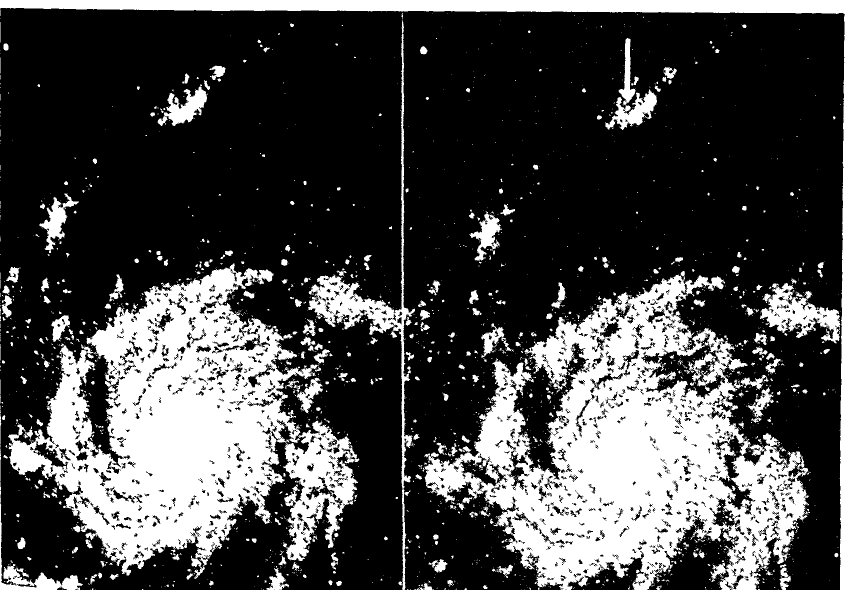
\includegraphics[width=\textwidth]{figures/chapter15/fig15-02.png}
  \par\vspace{0.25em}
  \makebox[\textwidth]{%
    \makebox[0.49\textwidth][c]{\small JUNE 9, 1950}\hfill
    \makebox[0.49\textwidth][c]{\small FEB.\ 7, 1951}%
  }
  \caption{Recent Supernova in the galaxy NGC5457 (M101); photographed with
  the 200-in.\ telescope at Mt.\ Palomar. (Courtesy Mt.\ Wilson and Mt.\
  Palomar observatories.)}
  \label{fig:15.2}
\end{figure}
\endgroup


At such short distances, we should replace \(z\) in Eq.~\eqref{eq:15.4.50}
by the small quantity \(H_0d\). Also, newborn pulsars would probably emit
about \(10^4\) pulses/sec, so we are here really interested in the difference
of the time delay at neighboring frequencies \(\nu_0\) and
\(\nu_0+\dd\nu_0\):
\[
  -\left(\frac{\dd\Delta t}{\dd\nu_0}\right)\dd\nu_0
  =
  \nu_{p0}^2\nu_0^{-3}\dd\nu_0\,d.
\]
For instance, if \(\nu_{p0}=31\,\mathrm{Hz}\), the difference in arrival
times of pulses from a pulsar in M101 at frequencies 1000 MHz and 1001 MHz
would be \(4\times10^{-4}\,\mathrm{sec}\), comparable with the expected
pulsar period. By working at 100 MHz rather than 1000 MHz, it would be
possible to detect electron densities as low as about
\(10^{-9}\,\mathrm{cm^{-3}}\). The problem will be to find a pulsar in some
other galaxy.

Other effects of an ionized intergalactic medium on light signals include
scintillation,\hyperref[ch15-ref-50a]{\textsuperscript{50a}} free-free
absorption,\hyperref[ch15-ref-50b]{\textsuperscript{50b}} and perhaps Faraday
rotation.\hyperref[ch15-ref-50c]{\textsuperscript{50c}} Only scintillation
now seems promising as a probe for the missing mass.
